\section{Second-hierarchy Tensor Embedding model} 

According to the extracting 5UD-CFG in the Section 4, this section discusses how we utilize the feature vector of 5UD-CFG embedding, compress and cluster them into a more concise feature that is suitable for achieving scalable and accurate app homology analysis. The second-hierarchy embedding process is the tensor embedding, which generates 3UD-CFG based on 5UD-CFG. 

\subsection{Tensor embedding model}
We propose a tensor embedding model for generating a more concise and effective feature vector. We review a well-studied factorization and compact model that are based on the first-hierarchy CFG embedding. In Definition 5, we can set $I_1$ of the second-hierarchy embedding tensor model firstly. For example, if the tensor embedding model is used to malware detection, we can set $I_1$ as the malware label of the app, $I_1$ can be defined as \emph{$I_1=1$ if this method is from the begin app, $I_1=0$ if this method is from the malware app,}
%Relationships among the number of CFG, the feature of CFG and the classification of CFG. 
%\begin{equation*}
% \begin{split}
%&I_1=\\
%\begin{matrix}
%1,~ if this method is from the begin apk\\
%0,~ if this method is from the malware apk \\
%\end{matrix}
%\end{split}
%\end{equation*}

%\begin{eqnarray*}\label{nn}
%\begin{cases}
% &I_1=1,~ if~this~method~is~from~the~begin~apk,\\
% &I_1=0,~ if~this~method~is~from~the ~malware~ apk.\\
%\end{cases}
%\end{eqnarray*}

%\begin{eqnarray*}
%	\begin{cases}
%		I_1=& 1, if this method is from the begin apk\\
%		& 0, if this method is from the malware apk.
%	\end{cases}
%\end{eqnarray*}

We use the accepted notation where an order-3 tensor is indexed by 3 indices and can be represented as a multidimensional array of data \cite{Kilmer2011Factorization}. That is, an order-3 tensor, $A$, can be written as 
\begin{equation}
	A=(a_{i_1i_2i_3})\in R^{n_1\times n_2\times n_3}~~(n_3=1).
\end{equation}

A third-order tensor can be pictured as a "cube" of data. It is convenient to refer to its slices. We use lateral slices to specify which two indices are held constant. Using the MATLAB notation, $A(:,k,1)$ corresponds to the k-th lateral slice. $A$ tube of a third-order tensor is defined by holding the first two indices fixed and varying the third. In particular, the third orientation of our tensor embedding model indicates a label. It does not join in the calculation of the tensor embedding model. 

As shown in the Fig. 3, we cut slices for the tensor embedding model expand in the horizontal orientation. 
\begin{figure}[hbt]
  \center{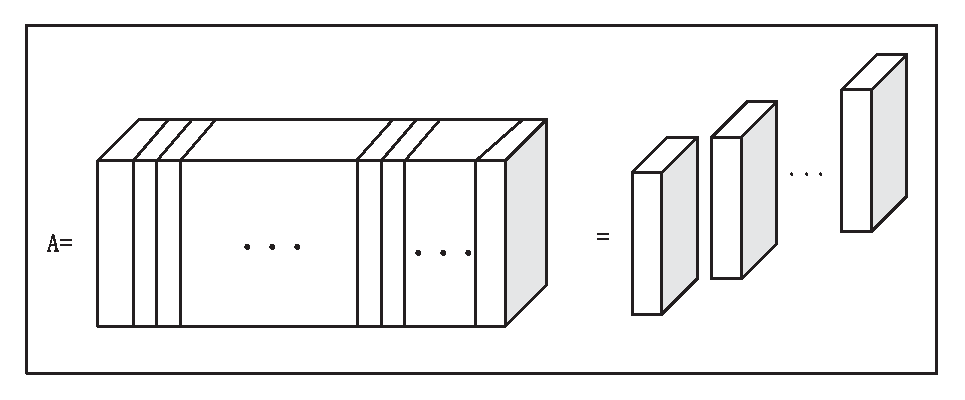
\includegraphics[width=8cm] {tensor.eps}}
  \caption{\label{1} Lateral slices of the tensor model $A$}
\end{figure}

For the third-order tensor embedding model, $A \in R_{n_1\times n_2 \times n_3}$, we have the representation that the tensor unfolding $A_{(3)}\in R^{I_f\times (I_n*1)}$ contains element $t_{i_1i_2}$ at the position with row number $f_i$ and column number $n_i$, $i_1$ is No. of the feature vector with five eigenvalues. $i_2$ is No. of the CFG. 

The following section, we will discuss how the function is decomposed in the tensor embedding model. 

\subsection{Compact 5UD-CFG to 3UD-CFG Based on tensor embedding model}
First we review the Singular Value Decomposition (SVD) \cite{Thomasian15} \cite{HanWZY18} as compressing algorithm for 5UD-CFG. An SVD of the tensor model that consists of all apps' 5UD-CFG embedding vector is $A=UDV^T$. We interpret the matrix $U$ to consist of latent embedding vectors in rows, for each entity represented in the first dimension of $A$. The matrix $A$ is constructed by a linear combination of the embedding $U$ with weights defines as rows of $(DV^T)^T$.

Then we consider $U=A(DV^T)^{\dagger}$, which is an inverse-relation, to be a mapping function from $A$ to the latent embedding in $U$. It is generally assumed that this mapping relation also holds for a new observation which is not present in $A$, i.e.
\begin{equation}
	u_{new}^T=x_{new}^T(DV^T)^{\dagger}.
\end{equation}

The first step in the proposed method is to unfold the scalable embedding tensor model. Similarly, we anchor the MatVec command \cite{DGaoCYWG17} to the lateral slices of the tensor, $MatVec(A)$ takes an $n_1\times n_2 \times n_3$ tensor and returns a block $n_1*n_3\times n_2$ matrix, in which model, $n_3=1$,
\begin{equation*}
 \begin{split}
&MatVec(A)=\left[
\begin{matrix}
c_1 \\
c_2 \\
\vdots \\
c_{n_2} \\
\end{matrix}
\right].
\end{split}
\end{equation*}

The operation that takes $MatVet(A)$ back to tensor form is the fold command:
\begin{equation}
  fold~(MatVet(A))=A.
\end{equation}

%We use the singular value decomposition \cite{ATensor5} and tensor decomposition \cite{ATensor6}.
The tensor mapping model defines a function $f(\bullet; \psi_l$) that maps each row in tensor unfolding $A^l$ to the corresponding row in the embedding matrix $X^l$ as 
\begin{equation}
	\widehat{A^l}=f(X^l; \psi_l)~ \forall l \in [1,..,L]. 
\end{equation}

Note that in the input of mapping function, each arbitrary row $i$ in $X_l$.

We define the mapping cost function as
\begin{equation}
    c_M=\sum_{l=1}^L d_M(A_l, \widehat{A_l})=\sum_{l=1}^L d_M(A_l, f(X_l; \Psi_l)).
\end{equation}

Optimizing that mapping cost function involves adjusting $\Psi_l$ for each $l$ with a given $f(\bullet)$ so that the distance between the learned embedding $A_l$ from factorization and mapped embedding $ \widehat{A_l}$ from the corresponding tensor unfolding is minimized.

Based on the SVD factorization \cite{DGorrell06} \cite{DChenC14} of proposed tensor model, we define $f(\bullet)=(DV^T)^T$. We embed all 5UD-CFGs into a smaller embedding vector called 3UD-CFG, which means compress 5UD-CFG embedding model. The core tensor and truncated bases of SVD decomposition described in the preliminaries can be employed to make considerable data smaller. In particular, for our tensor embedding model, the SVD factorization is as follows:

\textbf{Definition 6 [Singular Value Decomposition (SVD)] for our model:} Let $A\in R^{m\times tn\times 1}, m<tn$ denote a matrix, the factorization 
\begin{equation}
  A=USV^{T},
\end{equation}
is called the SVD of $A$. Matrices $U$ and $V$ refer to the left singular vector space and the right singular vector space of matrix $A$ respectively. Both $U$ and $V$ are unitary orthogonal matrices. Matrix $S=diag(\delta_1, \delta_2,...,\delta_k,...\delta_m)$ is a diagonal matrix that contains the singular values of $A$. In Section 3, we know that the number of extracted embedding vector is $m=5$, therefore, $k<5$, the smaller $k$ has more effective match, but the larger $k$ has more accurate match, we choose $k=2$ or $k=3$, the compression tensor model is as follows:

\begin{equation}
  M_k=U_kS_kV_k^{T},
\end{equation}
is called the rank-k truncated SVD of $A$, where $U_k=[u_1,u_2,...,u_k]$, $V_k=[v_1,v_2,...,v_k]$, $S_k=diag(\delta_1, \delta_2,..., \delta_k)$. The truncated SVD of $M$ is much smaller to store and faster to computer. We decompose the tensor model to classify the app, so we need to make the unitary orthogonal matrices $U$ as the projection and compressed orientation. 

We change tensor model $A\in R^{m\times tn \times 1}$ as a compressed tensor model $A \in R^{k\times tn\times 1}$. This process decreases original $m$ feature to particular $k$ feature $k<m$, which is called the feature compression. It is shown as the following equation:
\begin{equation}
  U^T_{k\times m}A_{m\times tn} \approx S_{k\times k} V^T_{k\times tn}.
\end{equation}

We obtain a mount of app features from app samples as the homology search database. Algorithm 1 shows the compression algorithm for 3TU-CFG tensor embedding model $A$ by the SVD factorization. %Before decomposing the tensor model by the SVD algorithm, we make the spare matrix centering by the fast Fourier transform. 

%\begin{algorithm}
%\caption{PSO}
%\label{pseudoPSO}
%\begin{algorithmic}[1]
%\State Initialize a population of particles with random values positions
%       and velocities from \textit{D} dimensions in the search space
%\While{Termination condition not reached}
%\For{Each particle $i$}
%    \State Adapt velocity of the particle using Equation \ref{eq:1}
%    \State Update the position of the particle using Equation \ref{eq:2}
%    \State Evaluate the fitness {$f(\overrightarrow{X}_i)$}
%    \If{$f(\overrightarrow{X}_i)<f(\overrightarrow{P}_i)$}
%       \State $\overrightarrow{P}_i \gets \overrightarrow{X}_i$
%    \EndIf
%    \If{$f(\overrightarrow{X}_i)<f(\overrightarrow{P}_g)$}
%       \State $\overrightarrow{P}_g \gets \overrightarrow{X}_i$
%    \EndIf
%\EndFor
%\EndWhile
%\end{algorithmic}
%\end{algorithm}

\begin {algorithm}
\caption{T-SVD-Compare}	
\begin{algorithmic}[1]
\Require~~
\State \textbf{Input}:
\State tensor model $A=R^{m\times tn}$, testing app feature set B;
%\State y=fft(A,[],1);
\State [U,S,V]=SVD(y);
%\State U1=ifft(U,[],1);
\State U2=U1(:,1:2);
\State T=real(U2'*A); compress feature
\State save T as the comparable object;
\State V1{}=clustering(V)
\State V3=centroid$\left\{V1\left\{ \right\}\right\}$ ~V3~ is ~the ~centroid~ vector~ in ~clustering~ set~ V1 $\left\{ \right\}$
\State A1=T*V3
\State A2{}=T*V1{}, 
\State B1=U2'*B compress detected app feature
\State B2=B1*V3
\State Compare (B2, B), ~get the closest element in the set V1{}
\State B3=B1*V1{the corresponding element}
\State Compare(B3, A2{the corresponding element})
\State \textbf{Output}:~The closest comparable result.
\end {algorithmic}
\end {algorithm}

In we present a compression strategy based on Algorithm 1, the compression is based on the assumption that the terms $||S(m,m,1)||_F^2$ decay rather quickly. A particularly nice feature of SVD compress proves that an optimal approximation of a tensor is closed to the original tensor. We prove the $A\approx A_k$ in our model as follows:
\begin{proof}

	First, we adopt the definition of the Frobenius norm of a tensor used in the literature:
	
	\textbf{Definition 7:} Suppose $A=a_{ij1}$ is size with $n_1 \times n_2 \times 1$, Then
		\begin{equation}
			||A||_F=\sqrt{\sum_{i=1}^{n_1} \sum_{j=2}^{n_2} a_{ij}^2}.
		\end{equation}
	
	We calculate he Frobenius norm between the original tensor and the approximate tensor as the mapping cost function $c_M$.
	\begin{equation*}
	\begin{split}
		&||A-A_k||_F^2=||USV^T-U_kS_kV_k^T||_F^2\\
		&=||S(k+1:m, K+1:m,1)||_F^2\\
		&=||F_m\times S(k+1:m, k+1,m)||_F^2\\
		&=||\delta_{k+1}||_F^2+||\delta_{k+2}||_F^2+...+||\delta_m||_F^2. \\
		&\leq T_{error}~~~(Error~~Threshold)		
	\end{split}
	\end{equation*}
	Since the singular value is decreasing in order and the difference between two neighbors is also greatly decreasing in order,  we choose the first three maximum singular values, the approximate tensor $U_kS_kV^T_k$ is closest to the original tensor model $A$.
\end{proof}

According to a mount of experiments, we can know the SVD factorization has the minimal error. The most major information are concentrated on the first several maximum singular values.
Therefore, $A\approx A_k$, when compressing the feature of 5UD-CfG, $(U'*A)(1:k,1:k,1)\approx (U_k'*A)$. The five feature of the 5UD-CFG is projected as major two or three features to nearly loselessly represent the original tensor model.


\subsection{Clustering of 3UD-CFG tensor embedding model}
After 5UD-CFG embedding model is decomposed as 3UD-CFG tensor embedding model by the SVD algorithm, we need to cluster the decomposing unitary orthogonal matrices $V_k$. The clustering result is generated from a training set of $S_k\times V_k$. The clustering result is as the app homology analysis basis. Each cluster comprises a number of closed 3UD-CFGs, which is community of similar CFG for apps.

In this paper, we use a k-means clustering as the unsupervised learning algorithm to generate the clustering result of the $S_k\times V_k$. Formally, the k-means clustering partition the training 3UD-CFG tensor embedding model into $t$ sets $SV=\left\{SV_1,SV_2,...,SV_t\right\}$ so as to minimize the sum of the distance of every 3UD-CFG to its cluster center. $c_i \in SV_c$ is the centroid for the subset $SV_i$, and the collections of all centroid nodes constitute the clustering center of the projected tensor $SV_c$. 

The number $t$ of the clustering will affect the search accuracy. Tensor factorization is effectively handle to the scalable data. We cluster all column vectors in $SV_k$. Then we get the above centroid set $SV_c$ and each clustering set $SV_c=\left\{SV_{c_1},SV_{c_2},...Sv_{c_t}\right\}$ as homology analysis data. First, we calculate the distance between the detected sample $B$ and the centroid set $SV_c$. We find indexes of the minimum two vector as the comparable candidate. This two indexes is denoted as $i,j$. Second, we calculate distance between each vector of the $SC_i$, the $SC_j$ and the detected sample $B$. Therefore, we get the closest distance with $B$ in $SC_i$ or $SC_j$. The process is as follows:
\begin{equation*}
\begin{split}
	 &\left\{SV_i,SV_j\right\}=arg~min_{i,j\in \left\{1,2...,t\right\} } distance~(B,SV_c)\\
	 &\longrightarrow object=arg~min_{SV_g\in (SV_i \bigcup SV_j)}distance ~(B, SV_g).\\
\end{split}
\end{equation*}

Object is the result that we want to get.

Comparison between $SV_c$, $SV_i$ or $SV_j$ and $B$ is a search problem. For high-dimension features in the machine learning, the most effective method to find the nearest neighbor is the randomized k-d forest and the priority search k-means tree, which is more effective than the LSH algorithm. This section introduces a scalable solution by the fast KNN search \cite{AntolD17}. The principle and major steps of the brute-force KNN search are as follows:

Considering a set $SV_c$ of $t$ reference points in a d-dimensional space $SV_c=\left\{SV_{c_1},SV_{c_2},~...,~Sv_{c_t}\right\}$, and a set $B$ of $q$ query points in the same space $B=\left\{b_1,b_2,...b_q\right\}$, for a query point $b\in B$, the brute-force algorithm is composed of the following steps:
1) Compute the distance between $b$ and $t$ reference points of $SV_c$; 2) Sort $t$ distances; 3) Output distances in the ordered of increasing distance.


When applying this algorithm for the $q$ query points with considering the typical case of large sets, the complexity of this algorithm contains two parts:$O~(tq)$ multiplication for the $tn\times m$ distances computed, $O~(tq~logt)$is for t sorting processes.

The brute-force kNN search method is by nature highly parallelizable and perfectly suitable for the high-dimension feature search.

In above methods, we use the clustering result of columns of $S_k$ multiply by $V_k$ to represent the clustering result of columns of original tensor model. Next we prove why the clustering result of columns of $S_k\times V_k$ can represent the clustering result of columns of $A$.

\begin{proof}
	We know that $U_k^T \times A= S_k \times V_k$ from the SVD decomposition of $A$. This means that we need to prove the clustering result of columns of $U_k^T \times A$ represents the clustering result of columns of $A$.
	
	Based on the SVD decomposition, we know that the $U_k$ is an orthogonal tensor $U_k\in R^{m\times k\times 1}$,
	\begin{equation}
		||A||^F_2=trace((A*A^T)_{(:,:1)}),
	\end{equation}
	where $(A*A^T)_{(:,:,1)}$ is the lateral slice of $A*A^T$ and $(A*A^T)_{(:,:,1)}$ is the lateral slice of $A^T *A$. Therefore,
	\begin{equation*}
		\begin{split}
			&||U_k^T*A||^F_2=trace([(U_k^T*A)^T*(U_k^T*A)]_{(:,:,1)})\\
			&=trace([A^T*U_k*U_k^T*A]_{(:,:,1)})\\
			&=||A||_F^2.
		\end{split}
	\end{equation*}
	
\end{proof}

We are finally in a position to consider tensor factorizations of 3UD-CFG tensor embedding model that are effectively handle the cluster and classification.

\subsection{Incremental tensor embedding for updating}

Based on the recursive incremental HOSVD proposed by the Liwei Kuang \cite{KuangHYLLM14} \cite{ZhaoYZ18}, we propose a incremental tensor model for the expanding app homology analysis model. The special steps is shown in the Algorithm. 2. 

\begin {algorithm}
\caption{T-SVD-Incremental}	
\begin{algorithmic}[1]
\Require~~
\State \textbf{Input}:
\State Initial tensor model $A_{i-1}$ and incremental 5UD-CFG feature matrix $C_{i-1}$.
\State Decomposition and compression results $U_{k_{i-1}},~S_{k_{i-1}},~V_{k_{i-1}}$ of tensor model $A_{i-1}$.
\State Project $C_{i-1}$ on the orthogonal space spanned by $U_{k_{i-1}}$, $Span=U_{k_{i-1}}^T\times C_{i-1}$.
\State Compute $H$ which is orthogonal to $U_j$, $H=C_{i-1}-U_{k_{i-1}}\times Span$
\State Obtain the unitary orthogonal basis $J$ from matrix $H$;
\State Compute the coordinates of matrix $H$, $K=J^T\times H$;
\State $[A_{i-1}, C_{i-1}]=[U_{k_{i-1}}, J] \left [\begin{matrix}
	S_{k_{i-1}}& J \\
	0 & K \\
\end{matrix}\right] \left[\begin{matrix}
	V&0\\
	0&I\\
\end{matrix}\right ]$
\State Obtain the unitary orthogonal basis $Uo,Vo$ from matrix $\left [\begin{matrix}
	S_{k_{i-1}}& J \\
	0 & K \\
\end{matrix}\right]$;
\State Obtain new decomposition results, $U=[U_{k_{i-1}}J]\times Uo, V=\left[\begin{matrix}
	V&0\\
	0&I\\
\end{matrix} \right]Vo$

\State \textbf{Output}:~U, ~V.
\end {algorithmic}
\end {algorithm}

We compute the incremental SVD decomposition method for streaming 5UD-CFG feature data dimensionality reduction. We just need the new decomposing unitary orthogonal matrix $U,~V$. This incremental algorithm only needs to decompose the incremental part $C_{i-1}$ rather than decomposing all matrix $[A_{i-1},C_{i-1}]$.







